\chapter{The Ionosphere}
\label{chapter:ionosphere}

The ionosphere is a section of Earth's atmosphere composed of several layers, between 60 and 1000\,km in altitude. It overlaps the Troposphere, Stratosphere, Mesosphere, Thermosphere and Exosphere. The ionosphere is an ionized plasma, composed of ions from molecules in the atmospheric layers it overlaps that are ionized by solar radiation. The ionization state of the ionosphere can be quantified by the Total Electron Content (TEC) -- an integral of electron count in a given direction -- among other metrics. 

Spatiotemporal variations of the TEC are tied to solar activity, and therefore largely both diurnal and seasonal. More ionization, and therefore a larger TEC, is to be expected in the day time and closer to the summer solstice. The Solar Cycle also influences TEC, with more sunspots proportional with a higher TEC; at solar maximum, this effect dominates the seasonal variation \citep{Sotomayor-Beltran.13}. Ionospheric variations are typically described as Kolmogorov turbulence (i.e. small scale motions are isotropic in their direction and scale with wavenumber; \citealt{Zolesi.14}), however, LOFAR observations report deviations from isotropy in their observations \citep{Intema.09, Mevius.16}. Regions of the ionosphere that can be assumed to be constant in density and shape at a given time are referred to as ``isoplanatic patches". At 74\,MHz, these patches are observed to be $1^{\circ}-2^{\circ}$ in radius \citep{Cotton.02}.

The ionosphere is composed of three main layers: D, E and F, which vary according to the day-night cycle. These are summarized in Section~\ref{tab:ionosphere_layers} (which summarizes Chapter 2 of \citealt{Zolesi.14}). At night, there are not enough high-energy electrons to penetrate to lower altitudes, causing the D layer to recombine. The E layer increases in altitude at night due to a similar effect. The E and F layers persist at all times, but during daylight the F layer is divided into two sub-layers, F$_1$ and F$_2$. 

\begin{deluxetable}{lllll}
\centering
\label{tab:ionosphere_layers}
\tablewidth{0pt}
\tablecaption{Ionospheric Layers}
\tabletypesize{\footnotesize}
\tablehead{
\colhead{Layer} & \colhead{Time} & \colhead{Altitude} &\colhead{Components} & \colhead{Electron Density}\\
\colhead{} & \colhead{} & \colhead{km} & \colhead{} & \colhead{$e^-\,m^{-3}$}
}
\startdata
D & Day & 60--90 & NO$^+$, N$_2$, Ar, O$_2^-$ & $10^8 - 10^9$  \\
E & Day/Night & 90--150 & NO$^+$, O$_2^+$, O$^+$, N$_2^+$ & $10^{11}$ \\
F$_1$ & Day & 140--600 & NO$^+$, O$_2^+$, O$^+$, N$^+$ & $10^{11}$\\
F$_2$ & Day/Night & 220--800 & O$^+$, H$^+$, He$^+$ & $10^{10} - 10^{13}$\\
\enddata
\end{deluxetable}

The diurnal nature of the ionosphere is important to radio propagation. During the day, the D layer reflects radio transmissions much closer to the Earth than during the night, when the E and F layers reflect. This leads to longer-range transmissions being possible after sunset\footnote{This effect was first observed by E. V. Appleton \citep{Appleton.46}, confirming the ionosphere's existence, for which he was awarded the 1947 Nobel Prize in Physics.}.

The relevance of the ionosphere to this work is its coupling with Earth's magnetic field. Recall that, as mentioned in previous chapters, a linearly polarized electromagnetic wave, propagating through an ionized plasma which has an incident magnetic field, will experience Faraday Rotation of its original polarization angle $\chi$:

\begin{equation}
\chi_{\rm obs} = \chi + \phi\lambda^2
\end{equation}

where $\lambda$ is the wavelength, and

\begin{equation}
\phi(\hat{s}) \approx 0.81 \int^{\rm obs}_{\rm source} n_e(\hat{s}) \vec{B}(\hat{s}) \cdot d\vec{s}
\label{eq:ionopshere_rm}
\end{equation}

where the source of the electromagnetic wave is in direction $\hat{s}$ on the sphere, $n_e$ is the electron density scalar field and $\vec{B}$ is the magnetic vector field. The Rotation Measure (RM) $\phi$ is the integral of the product along the line of sight, and has units of rad\,m$^-2$. Since the ionosphere is capable of imparting an additional RM to polarized radio waves, inducing spectral structure to interferometric visibilities, understanding it is crucial to quantifying the effect of polarization on EoR measurements.

In this chapter, I review historical measurements of the ionospheric TEC and RM distributions in Section~\ref{sec:historicalTEC} and modern observations in Section~\ref{sec:lowfreqionosphere}. In Section~\ref{sec:widefieldRMionosphere} I present our work on the role of the ionosphere in PAPER and HERA measurements, and software we developed to quantify those effects.

\section{Historical measurements of TEC and RMs}
\label{sec:historicalTEC}

The existence and layered nature of the ionosphere was confirmed between the 1920s and the 1940s. Measurements of the TEC and RM distributions came later, once radio-communications satellites were put in orbit, and are closely tied to the Global Positioning System (GPS) launched in the late 1970s (called the NAVSTAR system). NAVSTAR GPS satellites transmit at two narrow frequency bands, centered about 1.2276\,GHz (``L$_2$") and 1.57542\,GHz (``L$_1$"). Encoded in these transmissions are the local clock times per satellite (precisely calibrated with one another and with ground clocks) and their positions. With four satellites in view of a receiver, one is capable of computing their three-dimensional position and their local clock relative deviation from the satellite clock time. 

\cite{Macdoran.89} showed that one could use a frequency-dependent time delay induced by the ionospheric plasma \citep{Klobuchar.83, Brunner.93}:

\begin{equation}
\Delta t_{\rm iono} = \frac{40.3}{c\nu^2}{\rm TEC}
\label{eq:delta_iono}
\end{equation}

to calculate an estimate of the TEC in the direction of a GPS satellite. Their approach has been continously refined. 
Using an estimate of the polarization angle of the emitted L$_{1,2}$ transmissions, \cite{Titheridge.72} and \cite{Royden.84} presented measurements of TEC by measuring the Faraday Rotation induced and worked towards an estimate of the TEC based on the RM.
\cite{Lanyi.88} showed that the more accurate method was calculation of the TEC using $\Delta t_{\rm iono}$ from Equation~\ref{eq:delta_iono}.
\cite{Mannucci.98} introduced the Ionosphere Map Exchange Format (IONEX): a method and file format for storing TEC measurements using GPS beacons across the globe, allowing the first global TEC maps to be calculated. IONEX files contain global TEC measurements with a 2 hour cadence and generally 5$^\circ$ by 2.5$^\circ$ resolution in longitude and latitude respectively. They neglect the layered nature the ionosphere, modelling it as a thin sheet.
\cite{Iijima.99} provided a server that automatically pushed IONEX files to the World Wide Web as soon as they could be constructed.
\cite{Komjathy.05} presented the first measurements with over 1000 GPS stations.
Recently, \cite{Erdogan.16} presented a method for time-series forward modelling of the TEC distribution using IONEX files.

Meanwhile, many generations of the International Geomagnetic Reference Field \citep[IGRF][]{Finlay10} have continually improved the model of the Earth's magnetic field. This model is composed by spatial interpolation of magnetic field measurements (in up to 13th-order spherical harmonic coefficients) reported by institutions around the world.

Combining these two measurements -- IONEX and IGRF data -- can provide a map of RM distribution above any given position on Earth to moderate precision (better in the Northern Hemisphere than the Southern one, based on the number of GPS beacons in each). \cite{Afaraimovich.08} offered the first such software implementation, with the objective of using it to track Solar Activity\footnote{\cite{Erickson.01} were the first to present software capable of calculating ionospheric RMs using the IGRF, but they used local GPS beacons instead of IONEX files}. \cite{Sotomayor-Beltran.13} introduced the {\tt ionFR} package, which calculated ionospheric RMs towards a given position on the sky. We generalized their approach for the wide-field measurements in our {\tt radionopy} software package, which we present in Section~\ref{sec:widefieldRMionosphere}.

\section{Low frequency observations: discoveries and challenges}
\label{sec:lowfreqionosphere}

Low frequency interferometric observations are effected in two main ways by ionospheric turbulence: scintillation in Stokes I observations, and Faraday Rotation in Stokes Q and U observations. 

TEC variations introduce a variable index of refraction across a field of view. Stokes I signal from a point source will scintillate, change position, by an amount \citep[e.g.][]{TMS}:

\begin{equation}
\Delta\theta = - \frac{1}{8\pi^2} \frac{e^2}{\epsilon_0 m_e}\frac{1}{\nu^2} \nabla_{\perp}({\rm TEC})
\label{eq:ionosphere_scintillation}
\end{equation}

at the observed frequency $\nu$, where $\nabla_{\perp}$ is the transverse gradient in TEC towards the direction of the source. The time, space and frequency dependence of this effect causes difficulty for long integrations, since the scintillation will cause averaging of point sources with empty space, spreading-out their signal over a $\sim\Delta^2\theta$ area. This can be interpreted as an additional source of noise in a Stokes I map. \cite{Vedantham.15} showed that this scintillation noise can be much larger than image noise for baselines longer than $\sim 200$\,m. \cite{Vedantham.16}, extending the previous analysis to the Fourier domain, showed that this noise does not pose large issues to HERA or SKA-Low EoR efforts, since realistic amounts scintillation were not sufficient to wash-out EoR signals on large scales (their dense cores of relatively short baselines also help). However, it could pose large issues for point-source calibration and subtraction methods -- as emphasized in a public SKA memo by \cite{Cornwell.16}.

\cite{Loi.15} used MWA observation snapshots to map the scintillation as a function of space and time, resulting in the discovery of ``tubes" of plasma density waves across the Southern Hemisphere in lines of roughly constant latitude. Comparing the sources in their snapshot images to source positions in the NRAO VLA Sky Survey \citep[NVSS][]{Condon.98} they were able to calculate displacement vectors, and showed that they were strongly aligned to Earth's magnetic field.

The literature surrounding ionospheric Faraday Rotation is less extensive than work focussing on the unpolarized component. \cite{Lenc.16} showed that MWA measurements of diffuse foregrounds could provide a map of ionospheric spatiotemporal variance as their RM changed throughout a series of observations. \cite{Lenc.17} showed that point source power could be seen ``twinkling" in and out of polarized intensity maps due to ionospheric activity.

\section{Relevance for PAPER and HERA EoR measurements}
\label{sec:widefieldRMionosphere}

Within the PAPER and HERA power spectrum pipelines, many tens to hundreds of days of visibilities are averaged over during binning in LST. The the ionosphere-induced spatial and temporal fluctuations in RM could produce sufficient phase scrambling of the celestial Faraday-rotated, polarized signal to suppress a fraction of any polarized signal leaked by some mechanism into Stokes I measurements. The fringe size of the 30\,m baselines used in power spectrum analyses is large enough that scintillation effects are negligible.

This effect was first investigated in \cite{Moore.17}. Using the {\tt ionFR} package \citep{Sotomayor-Beltran.13} we calculated the RM distribution at a single zenithal pointing throughout the PAPER-32 observation season. This was a vast simplification given the PAPER primary beam was much larger than a typical isoplanatic patch. Shown in Figure~\ref{fig:ionosphere_psa32hist}, there was a large spread of ionospheric RMs for each LST. There was a decrease in the average magnitude of the RM as LST increased. This was expected, given the strong correlation between the day/night cycle and TEC values \citep[e.g.][]{Tariku.15}, and given that for this observing season, LST=4 hr corresponded to observations taken shortly after sunset, while LST=8 hr was always well into the night.

\begin{figure}
\centering
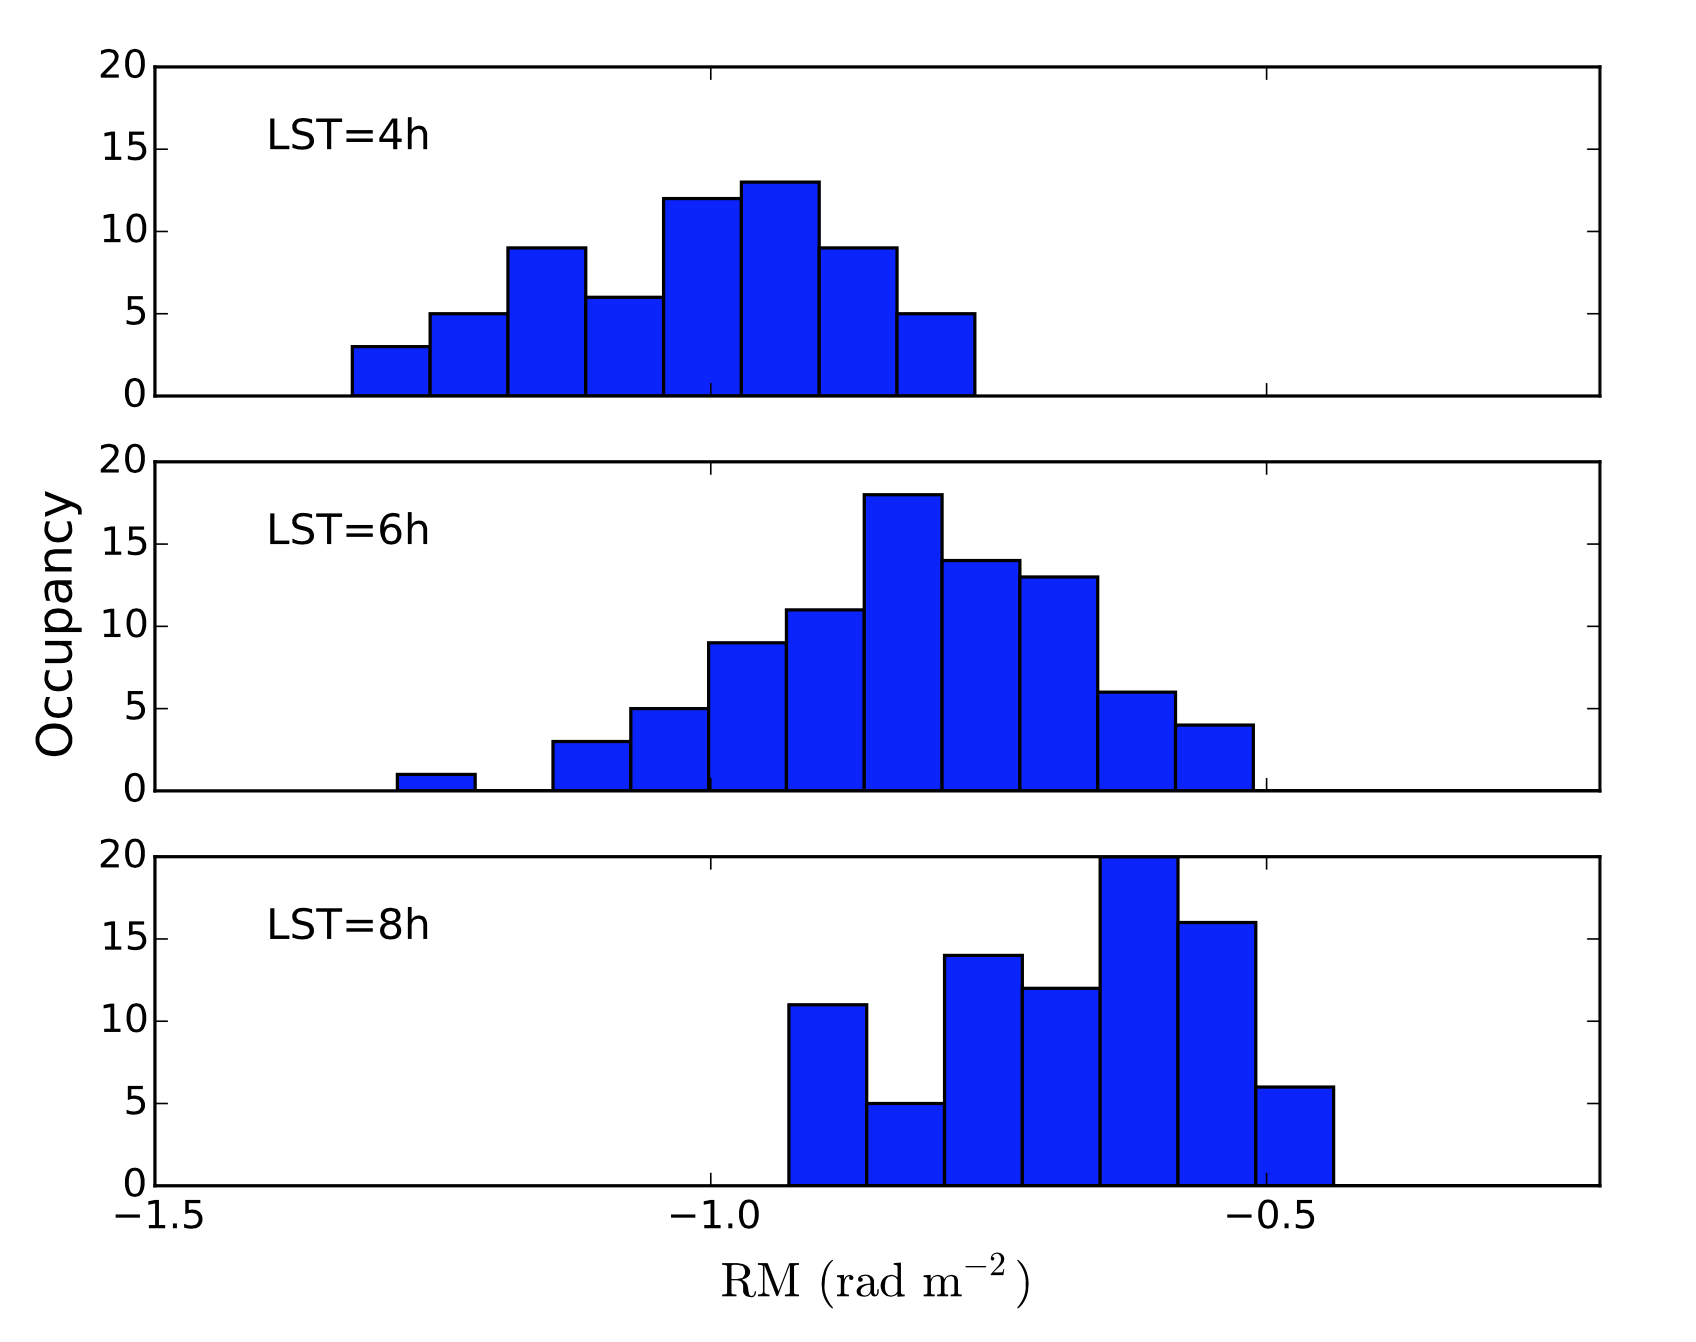
\includegraphics[width=0.9\textwidth]{chapters/ionosphere/figures/MooreHist.png}
\caption[Distribution of zenithal ionospheric RMs for 3 LSTs in the PAPER-32 observing season]{Distribution of zenithal ionospheric RMs for 3 LSTs in the PAPER-32 observing season. From top to bottom: a histogram of the zenith ionospheric RMs over the season, for the transit of LSTs 4, 6, and 8 hr. Taken from \cite{Moore.17}.}
\label{fig:ionosphere_psa32hist}
\end{figure}

Treating the single pointing as constant over the sky, we calculated the expected attenuation of polarized signal, leaked into pseudo-Stokes I visibilities, that would be averaged over varying ionospheric conditions during LST binning. These attenuation factors were 43$\pm$6\% at 165\,MHz and 7$\pm$5\% at 126\,MHz.

To build on this result, we required more sophisticated simulations of the interaction of the polarized sky with the instrument and whole-sky maps of the ionosphere. To accomplish the latter, we developed the open-source Python package {\tt radionopy}\footnote{\url{https://github.com/UPennEoR/radionopy}}. Like {\tt ionFR}, {\tt radionopy} uses GPS-derived TEC maps from IONEX files and the IGRF to estimate the value of ionospheric RM at a given latitude, longitude and date. Unlike its predecessor, {\tt radionopy} does not necessarily calculate an RM at a given pointing, but instead is capable of calculating the ionospheric RM over a {\tt HEALPix} grid of the sky \citep{Gorski.05}. Such an expression of ionospheric variation is natural to wide-field, drift-scanning EoR arrays, and reflects the format of the IONEX input measurements, which are given in their spherical harmonic decompositions. {\tt radionopy} is vectorized, leading to efficient generation of full-sky ionospheric maps, and object-oriented, allowing for easier collaborative development. Additionally we implemented the interpolation scheme recommended in the IONEX documentation to obtain ``best-guess" full-sky maps for arbitrary times between the 2-hour time resolution of IONEX data. 

An example output from {\tt radionopy} is shown in Figure~\ref{fig:ionosphere_radionopy_example} as a {\sc HEALPix} grid of the hemisphere observable from the PAPER site in the Karoo. In Figure~\ref{fig:ionfr_compare} we show {\tt radionopy} and {\tt ionFR} output for a single pointing towards Cassiopeia A (Cas A; RA=23$^{\rm h}$23$^{\rm m}$27.9$^{\rm s}$, Dec=$+58^{\circ}48'42.4''$) from the LOFAR Core site in the Netherlands. The two codes gave qualitative agreement. Slight offsets at the highest RM values that day could be attributed to differences in our interpolation schemes.

\begin{figure}
\centering
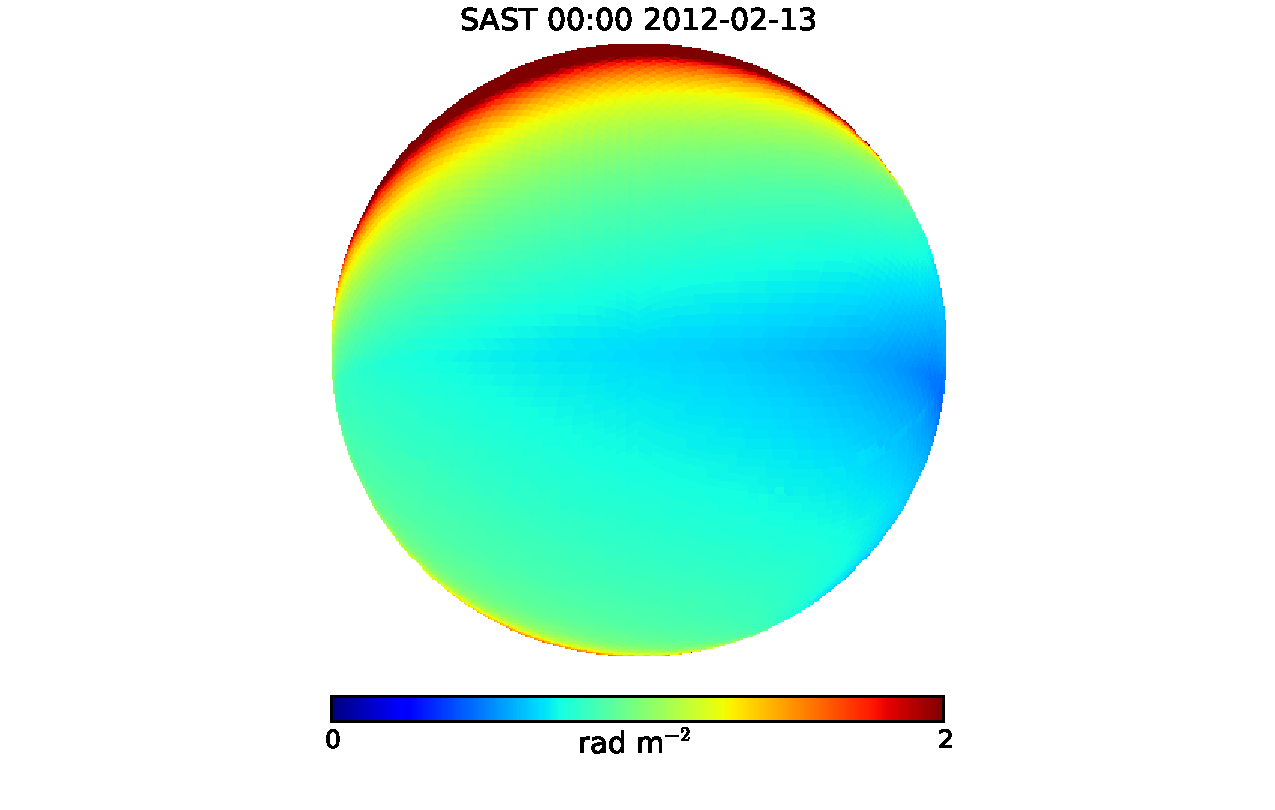
\includegraphics[width=0.9\textwidth]{chapters/ionosphere/figures/widefield_RM_snap.pdf}
\caption{An example of widefield ionospheric RMs calculated by {\tt radionopy}.}
\label{fig:ionosphere_radionopy_example}
\end{figure}

\begin{figure}
\centering
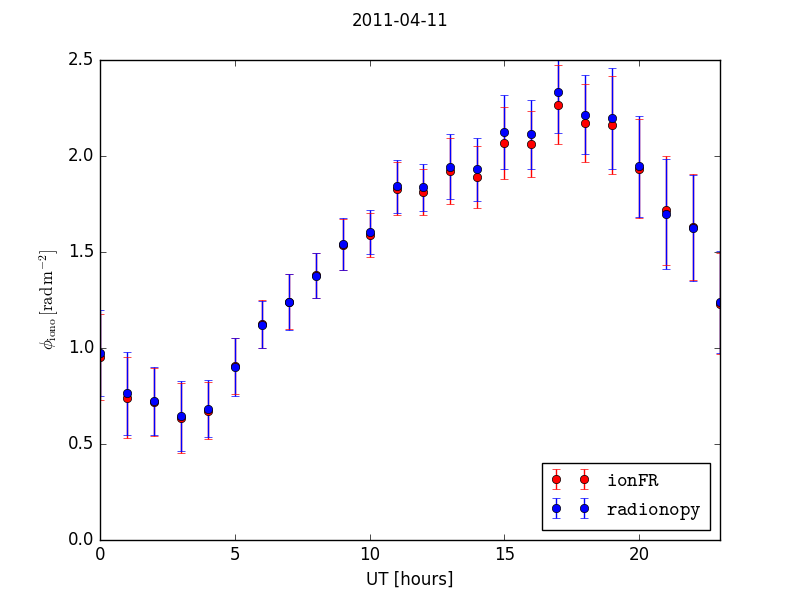
\includegraphics[width=0.9\textwidth]{chapters/ionosphere/figures/ionFRcompare.png}
\caption[The RM of Cas A as viewed from the LOFAR Core site in the Netherlands on April 11th, 2011, according to {\tt ionFR} and {\tt radionopy}.]{The RM of Cas A as viewed from the LOFAR Core site in the Netherlands on April 11th, 2011, according to {\tt ionFR} and {\tt radionopy}. The two codes show quantitative agreement, demonstrating that radionopy can be used for single-pointing as well as full-sky RM measurements.}
\label{fig:ionfr_compare}
\end{figure}

{\color{red}Martinot et al. (in prep.)} investigated the full interaction of the polarized sky with the ionosphere, using realistic polarized sky models and fully-polarized HERA beam models (see Chapter~\ref{chapter:eor_window_HERA} for an example). Their work revealed that the \cite{Moore.17} analysis overestimated the ionospheric attenuation due to their single-pointing and simple beam models. Realistic levels of attenuation for a 100 day HERA integration can be expected to reach a factor of $\leqslant 0.1$. If polarization leakage occurs close to the EoR level, this is sufficient to recover the EoR power spectrum. However, if it is above the EoR level (as expected by \citealt{Nunhokee.17}), the ionosphere alone will not be sufficient to rule out polarization leakage being detected before the EoR can be recovered.
